\section{Result}

\begin{figure}[!ht]
  \centering
  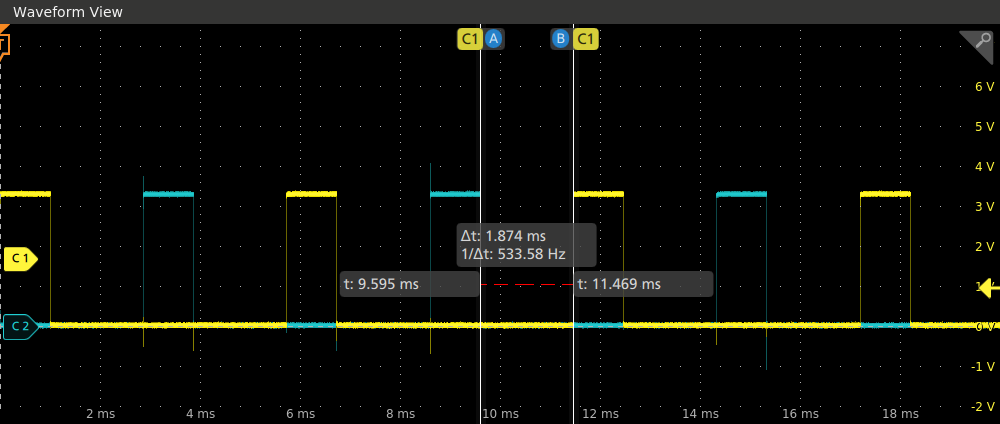
\includegraphics[scale=0.5]{assets/framework-value-wave.png}
  \caption{\label{fig:framework-value-wave}Voltage measurement of the two GPIOs; Each color represents a task}
\end{figure}

\begin{table}[!ht]
  \centering
  \begin{tabular}{llll}
                        & \multicolumn{3}{c}{Time ($\mu$s)}                             \\ \cline{2-4} 
                        & \multicolumn{1}{c}{Mean} & Min  & \multicolumn{1}{c}{Max} \\ \cline{2-4} 
  From task 1 to task 2 & 1864                     & 1863 & 1866                    \\
  From task 2 to task 1 & 1865                     & 1862 & 1866                    \\
  Duration of task 1    & 1003                     & 1003 & 1003                    \\
  Duration of task 2    & 1003                     & 1003 & 1003                   
  \end{tabular}
  \caption{Context switching times and task durations measured with the oscilloscope Tektronix MSO 56 using our framework}
  \label{tab:framework-measurement}
\end{table}

\subsection{Comparison with the reference measurement}

\begin{table}[!ht]
  \centering
  \begin{tabular}{lll}
                        & \multicolumn{2}{c}{Time ($\mu$s)}                                     \\ \cline{2-3} 
                        & \multicolumn{1}{c}{Reference} & Framework \\ \cline{2-3} 
  From task 1 to task 2 & 14.68                                     & 1864                  \\
  From task 2 to task 1 & 14.88                                     & 1865                  \\
  Duration of task 1    & 1003                                      & 1003                  \\
  Duration of task 2    & 1003                                      & 1003                 
  \end{tabular}
  \caption{Comparison}
  \label{tab:measurements-comparison}
\end{table}


\subsection{Limitations of the framework}
% As the next chapter explains, this framework idea encountered several limitations.
% First, the devices does not have enough internal power to compute the context switching time or the interrupt latency with engough precision.
% Second, we did not had enough time to build a framework able to measure the memory usage or the energy consumption.

\paragraph{Framework overhead}

\paragraph{Precision}